协程库、模块化标准库和执行器都是C++23的一部分。


\subsubsubsection{8.1.1\hspace{0.2cm}协程库}

C++20中的协程只不过是实现具体协程的框架,所以需要软件开发人员来实现协同程序。Lewis Baker的\href{https://github.com/lewissbaker/cppcoro}{cppcoro}库给出了协程库的第一个概念,该库提供了C++20没有的“高级协程”。

\begin{tcolorbox}[breakable,enhanced jigsaw,colback=blue!5!white,colframe=blue!75!black,title={使用cppcoro}]
	
cppcoro库是基于协程TS的。TS代表技术规范,是C++20所提供的协程功能的初步版本。Lewis大概会将cppcoro库从协程TS移植为C++20中定义的协程。该库可以在Windows (Visual Studio 2017)或Linux (Clang 5.0/6.0和libc++)上使用。在我的实验中,对所有示例都使用了以下命令行:

\hspace*{\fill} \\ %插入空行
\noindent
\textbf{cppcoro的命令行}
\begin{tcblisting}{commandshell={}}
clang++ -std=c++17 -fcoroutines-ts -Iinclude -stdlib=libc++ libcppcoro.a
  cppcoroTask.cpp -pthread
\end{tcblisting}

\begin{itemize}
\item 
-std=c++17: 支持C++17

\item 
-fcoroutines-ts : 支持C++协程TS

\item 
-Iinclude : cppcoro头文件

\item 
-stdlib=libc++: \href{https://en.wikipedia.org/wiki/LLVM}{LLVM}标准库的实现

\item 
libcppcoro.a: cppcoro库
\end{itemize}

正如我所说,当cppcoro基于C++20的协程时,就可以将它们用于支持C++20的编译器。此外,它们还让你对C++23中的具体协程实现有了初步了解。

本节关于协程库的其余部分中,我想演示几个示例,以展示协程的强大。我的演示从协程的类型开始。

\end{tcolorbox}

\hspace*{\fill} \\ %插入空行
\noindent
\textbf{8.1.1.1\hspace{0.2cm}协程的类型}

cppcoro具有很多生成器,可以执行有各种各样的任务(task)。

\hspace*{\fill} \\ %插入空行
\noindent
\textbf{8.1.1.1.1\hspace{0.2cm}task<T>}

什么是任务(task)?cppcoro中使用的定义是:

\begin{itemize}
\item 
任务表示延迟执行的异步计算,其中协程的执行直到等待任务时才开始。
\end{itemize}

任务是一个协程。在下面的程序中,函数main首先等待函数,第一个等待第二个,第二个等待第三个。

\begin{lstlisting}[style=styleCXX]
// cppcoroTask.cpp

#include <chrono>
#include <iostream>
#include <string>
#include <thread>

#include <cppcoro/sync_wait.hpp>
#include <cppcoro/task.hpp>

using std::chrono::high_resolution_clock;
using std::chrono::time_point;
using std::chrono::duration;

using namespace std::chrono_literals;

auto getTimeSince(const time_point<high_resolution_clock>& start) {

	auto end = high_resolution_clock::now();
	duration<double> elapsed = end - start;
	return elapsed.count();

}

cppcoro::task<> third(const time_point<high_resolution_clock>& start) {
	
	std::this_thread::sleep_for(1s);
	std::cout << "Third waited " << getTimeSince(start) << " seconds." << '\n';
	
	co_return;

}

cppcoro::task<> second(const time_point<high_resolution_clock>& start) {

	auto thi = third(start);
	std::this_thread::sleep_for(1s);
	co_await thi;
	
	std::cout << "Second waited " << getTimeSince(start) << " seconds." << '\n';

}

cppcoro::task<> first(const time_point<high_resolution_clock>& start) {

	auto sec = second(start);
	std::this_thread::sleep_for(1s);
	co_await sec;
	
	std::cout << "First waited " << getTimeSince(start) << " seconds." << '\n';

}

int main() {

	std::cout << '\n';
	
	auto start = high_resolution_clock::now();
	cppcoro::sync_wait(first(start));
	
	std::cout << "Main waited " << getTimeSince(start) << " seconds." << '\n';
	
	std::cout << '\n';

}
\end{lstlisting}

诚然,这个程序没有做什么有意义的事情,但它有助于理解协同程序的工作流程。

首先,主函数不能是协程。Cppcoro::sync\_wait(第59行)通常用作启动顶级任务,并等待任务完成。与其他协程类似,协程首先获取开始时间作为参数,并显示其执行时间。协程首先做什么?第二次启动协程(第36和46行),立即暂停,休眠一秒,然后通过句柄sec恢复协程(第38和48行)。第二个协程执行相同的工作流,但第三个协程不执行。至于第三个,它是一个协程,不返回任何东西,也不等待另一个协程。当第三个完成时,所有其他协程都会执行。因此,每个协程需要3秒。

\begin{center}
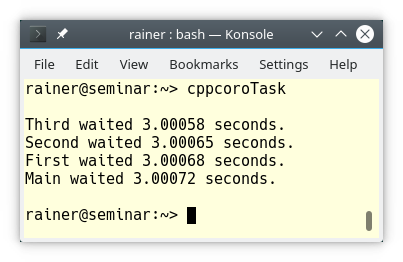
\includegraphics[width=0.8\textwidth]{content/5/chapter8/images/1.png}\\
\end{center}

稍微改变一下程序。若协程在co\_await调用后休眠会发生什么?

\begin{lstlisting}[style=styleCXX]
// cppcoroTask2.cpp

#include <chrono>
#include <iostream>
#include <string>
#include <thread>

#include <cppcoro/sync_wait.hpp>
#include <cppcoro/task.hpp>

using std::chrono::high_resolution_clock;
using std::chrono::time_point;
using std::chrono::duration;

using namespace std::chrono_literals;

auto getTimeSince(const time_point<::high_resolution_clock>& start) {

	auto end = high_resolution_clock::now();
	duration<double> elapsed = end - start;
	return elapsed.count();

}
cppcoro::task<> third(const time_point<high_resolution_clock>& start) {

	std::cout << "Third waited " << getTimeSince(start) << " seconds." << '\n';
	std::this_thread::sleep_for(1s);
	co_return;

}

cppcoro::task<> second(const time_point<high_resolution_clock>& start) {

	auto thi = third(start);
	co_await thi;
	
	std::cout << "Second waited " << getTimeSince(start) << " seconds." << '\n';
	std::this_thread::sleep_for(1s);

}

cppcoro::task<> first(const time_point<high_resolution_clock>& start) {

	auto sec = second(start);
	co_await sec;
	
	std::cout << "First waited " << getTimeSince(start) << " seconds." << '\n';
	std::this_thread::sleep_for(1s);

}

int main() {

	std::cout << '\n';
	
	auto start = ::high_resolution_clock::now();
	
	cppcoro::sync_wait(first(start));
	
	std::cout << "Main waited " << getTimeSince(start) << " seconds." << '\n';
	
	std::cout << '\n';

}
\end{lstlisting}

你可能已经猜到了。主函数等待3秒,但每个迭代调用的协程要少等待1秒。

cppcoro提供的下一个协程是generator<T>。

\hspace*{\fill} \\ %插入空行
\noindent
\textbf{8.1.1.1.2\hspace{0.2cm}generator<T>}

以下是cppcoro对生成器的定义:

\begin{itemize}
\item 
生成器表示生成T类型值序列的协程类型,其中的值是惰性和同步生成的。
\end{itemize}

话不多说,cppcoroGenerator.cpp程序演示了两个实际运行的生成器。

\begin{lstlisting}[style=styleCXX]
// cppcoroGenerator.cpp

#include <iostream>
#include <cppcoro/generator.hpp>

cppcoro::generator<char> hello() {
	co_yield 'h';
	co_yield 'e';
	co_yield 'l';
	co_yield 'l';
	co_yield 'o';
}

cppcoro::generator<const long long> fibonacci() {
	long long a = 0;
	long long b = 1;
	while (true) {
		co_yield b;
		auto tmp = a;
		a = b;
		b += tmp;
	}
}

int main() {

	std::cout << '\n';
	for (auto c: hello()) std::cout << c;
	
	std::cout << "\n\n";
	
	for (auto i: fibonacci()) {
		if (i > 1'000'000) break;
		std::cout << i << " ";
	}
	
	std::cout << "\n\n";

}
\end{lstlisting}

第一个协程hello应请求返回下一个字符,协程fibonacci返回下一个fibonacci数字。斐波那契数列可以创建无限的数据流。第33行发生了什么呢?基于范围的for循环触发协程的执行。第一次迭代启动协程,返回co\_yield b处的值(第18行),然后暂停。后续基于范围的for循环调用恢复协程fibonacci并返回下一个fibonacci数字。

\begin{center}
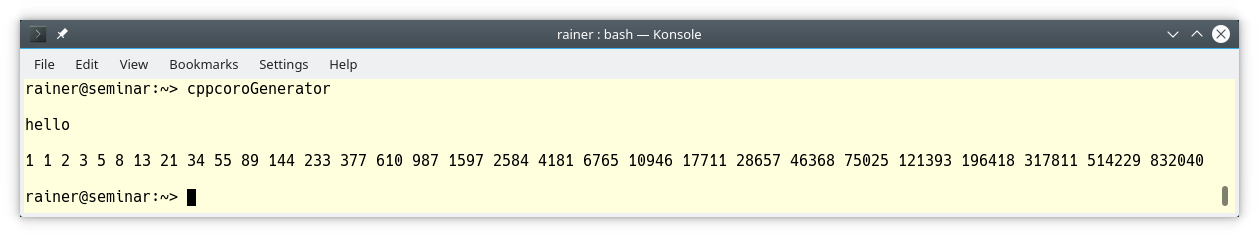
\includegraphics[width=0.8\textwidth]{content/5/chapter8/images/2.png}\\
\end{center}

cppcoro中提供了更多可等待的类型。

\hspace*{\fill} \\ %插入空行
\noindent
\textbf{8.1.1.2\hspace{0.2cm}可等待类型}

cppcoro支持各种可等待类型:

\begin{itemize}
\item 
single\_consumer\_event

\item 
single\_consumer\_async\_auto\_reset\_event

\item 
async\_mutex

\item 
async\_manual\_reset\_event

\item 
async\_auto\_reset\_event

\item 
async\_latch

\item 
sequence\_barrier

\item 
multi\_producer\_sequencer

\item 
single\_producer\_sequencer
\end{itemize}

我想仔细聊聊可等待的single\_consumer\_event和async\_mutex。

\hspace*{\fill} \\ %插入空行
\noindent
\textbf{8.1.1.2.1\hspace{0.2cm}single\_consumer\_event}

根据文档,single\_consumer\_event是一个手动重置事件类型,一次只支持单个协程的等待。single\_consumer\_event为线程的一次性同步提供了一种新方法。

\begin{lstlisting}[style=styleCXX]
// cppcoroProducerConsumer.cpp

#include <cppcoro/single_consumer_event.hpp>
#include <cppcoro/sync_wait.hpp>
#include <cppcoro/task.hpp>

#include <future>
#include <iostream>
#include <string>
#include <thread>
#include <chrono>

cppcoro::single_consumer_event event;

cppcoro::task<> consumer() {

	auto start = std::chrono::high_resolution_clock::now();
	
	co_await event; // suspended until some thread calls event.set()
	
	auto end = std::chrono::high_resolution_clock::now();
	std::chrono::duration<double> elapsed = end - start;
	std::cout << "Consumer waited " << elapsed.count() << " seconds." << '\n';
	
	co_return;
}

void producer() {

	using namespace std::chrono_literals;
	std::this_thread::sleep_for(2s);
	
	event.set(); // resumes the consumer

}

int main() {

	std::cout << '\n';
	
	auto con = std::async([]{ cppcoro::sync_wait(consumer()); });
	auto prod = std::async(producer);
	
	con.get(), prod.get();
	
	std::cout << '\n';

}
\end{lstlisting}

代码是自解释的。消费者(第41行)和生产者(第42行)在各自的线程中运行。因为主函数不能是协程,所以cppcoro::sync\_wait(consumer())调用(第41行)作为顶级任务。调用一直等待,直到协程使用者完成。协程消费者在调用co\_await事件(第19行)中等待,直到有人调用event.set()(第33行)。函数生产者在休眠两秒后发送它的事件。

\begin{center}
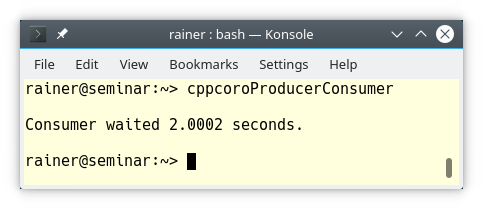
\includegraphics[width=0.8\textwidth]{content/5/chapter8/images/3.png}\\
\end{center}

cppcoro还支持\href{https://en.cppreference.com/w/cpp/named_req/Mutex}{mutex}。

\hspace*{\fill} \\ %插入空行
\noindent
\textbf{8.1.1.2.2\hspace{0.2cm}async\_mutex}

像cppcoro::async\_mutex这样的互斥锁是一种同步机制,多个线程中只有一个能够访问保护的共享数据。

\begin{lstlisting}[style=styleCXX]
// cppcoroMutex.cpp

#include <cppcoro/async_mutex.hpp>
#include <cppcoro/sync_wait.hpp>
#include <cppcoro/task.hpp>

#include <iostream>
#include <thread>
#include <vector>


cppcoro::async_mutex mutex;

int sum{};

cppcoro::task<> addToSum(int num) {
	cppcoro::async_mutex_lock lockSum = co_await mutex.scoped_lock_async();
	sum += num;

}

int main() {

	std::cout << '\n';
	
	std::vector<std::thread> vec(10);
	
	for(auto& thr: vec) {
		thr = std::thread([]{
		for(int n = 0; n < 10; ++n) cppcoro::sync_wait(addToSum(n)); } );
	}
	
	for(auto& thr: vec) thr.join();
	
	std::cout << "sum: " << sum << '\n';
	
	std::cout << '\n';

}
\end{lstlisting}

第26行创建10个线程,每个线程将数字0到9添加到共享sum变量(第14行)。addToSum函数是协程,在表达式co\_await mutex.scoped\_lock\_async()(第17行)中等待,直到获得互斥量。等待互斥锁的协程不是阻塞状态,而是挂起状态。前一个锁持有者在其解锁调用中恢复等待协程,所以互斥锁一直保持锁定状态,直到作用域结束(第20行)。

\begin{center}
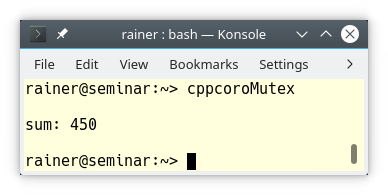
\includegraphics[width=0.8\textwidth]{content/5/chapter8/images/4.png}\\
\end{center}

\hspace*{\fill} \\ %插入空行
\noindent
\textbf{8.1.1.3\hspace{0.2cm}函数}

还有更有趣的函数可以用来处理可等待对象。

\begin{itemize}
\item 
sync\_wait()

\item 
when\_all()

\item 
when\_all\_ready()

\item 
fmap()

\item 
schedule\_on()

\item 
resume\_on()
\end{itemize}

when\_all函数创建一个等待所有输入可等待对象的可等待对象,并返回它们各自结果的聚合。

看看下面的代码,有个第一印象:

\begin{lstlisting}[style=styleCXX]
// cppcoroWhenAll.cpp

#include <chrono>
#include <iostream>
#include <thread>

#include <cppcoro/sync_wait.hpp>
#include <cppcoro/task.hpp>
#include <cppcoro/when_all.hpp>

using namespace std::chrono_literals;

cppcoro::task<std::string> getFirst() {
	std::this_thread::sleep_for(1s);
	co_return "First";
}

cppcoro::task<std::string> getSecond() {
	std::this_thread::sleep_for(1s);
	co_return "Second";
}

cppcoro::task<std::string> getThird() {
	std::this_thread::sleep_for(1s);
	co_return "Third";
}


cppcoro::task<> runAll() {

	auto[fir, sec, thi] = co_await cppcoro::when_all(getFirst(), getSecond(),
	getThird());
	
	std::cout << fir << " " << sec << " " << thi << '\n';

}

int main() {

	std::cout << '\n';
	
	auto start = std::chrono::steady_clock::now();
	
	cppcoro::sync_wait(runAll());
	
	std::cout << '\n';
	
	auto end = std::chrono::high_resolution_clock::now();
	std::chrono::duration<double> elapsed = end - start;
	std::cout << "Execution time " << elapsed.count() << " seconds." << '\n';
	
	std::cout << '\n';

}
\end{lstlisting}

顶层任务cppcoro::sync\_wait(runAll())(第44行)等待可等待的runAll,后者等待可等待的getFirst、getSecond和getThird(第31行)。可等待的runAll、getFirst、getSecond和getThird是协程。每个get函数休眠一秒钟(第14、19和24行),三乘以一秒等于三秒。这是调用cppcoro::sync\_wait(runAll())等待协程的时间,第49行显示时间持续时间。

\begin{center}
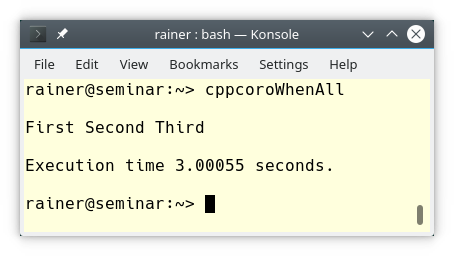
\includegraphics[width=0.8\textwidth]{content/5/chapter8/images/5.png}\\
\end{center}

可以将cpp中的when\_all和线程池结合起来

\hspace*{\fill} \\ %插入空行
\noindent
\textbf{8.1.1.4\hspace{0.2cm}static\_thread\_pool}

static\_thead\_pool在固定大小的线程池上进行调度工作。

可以调用cppcoro::static\_thread\_pool,也可以不调用。这个数字表示创建的线程数。若不指定数字,则使用C++11中加入的std::thread::hardware\_concurrency()。\href{https://en.cppreference.com/w/cpp/thread/thread/hardware_concurrency}{std::thread::hardware\_concurrency}给出了系统支持的硬件线程数,这可能是处理器或内核的数量。

来试试看。下面的示例基于cppcoroWhenAll.cpp,使用了可等待的when\_any。这一次,协程并发执行。

\begin{lstlisting}[style=styleCXX]
// cppcoroWhenAllOnThreadPool.cpp

#include <chrono>
#include <iostream>
#include <thread>

#include <cppcoro/sync_wait.hpp>
#include <cppcoro/task.hpp>
#include <cppcoro/static_thread_pool.hpp>
#include <cppcoro/when_all.hpp>


using namespace std::chrono_literals;

cppcoro::task<std::string> getFirst() {
	std::this_thread::sleep_for(1s);
	co_return "First";
}

cppcoro::task<std::string> getSecond() {
	std::this_thread::sleep_for(1s);
	co_return "Second";
}

cppcoro::task<std::string> getThird() {
	std::this_thread::sleep_for(1s);
	co_return "Third";
}

template <typename Func>
cppcoro::task<std::string> runOnThreadPool(cppcoro::static_thread_pool& tp,
                                           Func func) {
	co_await tp.schedule();
	auto res = co_await func();
	co_return res;
}

cppcoro::task<> runAll(cppcoro::static_thread_pool& tp) {

	auto[fir, sec, thi] = co_await cppcoro::when_all(
		runOnThreadPool(tp, getFirst),
		runOnThreadPool(tp, getSecond),
		runOnThreadPool(tp, getThird));
	
	std::cout << fir << " " << sec << " " << thi << '\n';

}

int main() {

	std::cout << '\n';
	
	auto start = std::chrono::steady_clock::now();
	
	cppcoro::static_thread_pool tp;
	cppcoro::sync_wait(runAll(tp));
	
	std::cout << '\n';
	
	auto end = std::chrono::high_resolution_clock::now();
	std::chrono::duration<double> elapsed = end - start;
	std::cout << "Execution time " << elapsed.count() << " seconds." << '\n';
	
	std::cout << '\n';

}
\end{lstlisting}

这是与之前的程序cppcoroWhenAll.cpp的关键区别。第55行,创建了一个线程池tp,并将其用作函数runAll(tp)的参数(第56行)。函数runAll使用线程池并发地启动协程,因为有了结构化绑定(第40行),每个协程的值可以很容易地聚合并分配给一个变量。最后,main函数只需要1秒而不是3秒。

\begin{center}
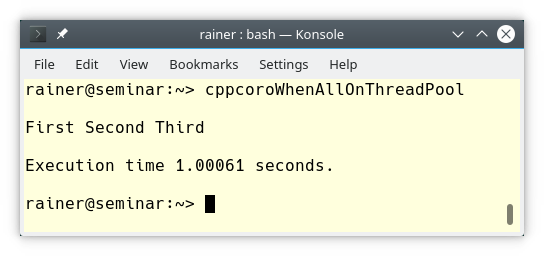
\includegraphics[width=0.8\textwidth]{content/5/chapter8/images/6.png}\\
\end{center}

\subsubsubsection{8.1.2\hspace{0.2cm}模块化的标准库}

也许您想停止使用标准库头文件?Microsoft根据C++提案\href{http://www.open-std.org/JTC1/SC22/WG21/docs/papers/2017/p0581r0.pdf}{P0541}支持所有STL头文件的模块。Microsoft的实现可以让开发者初步了解模块化的标准库是什么样的。以下是我在Microsoft C++团队博客的帖子\href{https://devblogs.microsoft.com/cppblog/cpp-modules-in-visual-studio-2017/}{Visual Studio 2017中使用C++模块}中找到的内容。

\hspace*{\fill} \\ %插入空行
\noindent
\textbf{8.1.2.1\hspace{0.2cm}Visual Studio 2017中使用C++模块}

\begin{itemize}
\item 
std.regex提供了头文件<regex>的内容

\item 
std.filesystem提供了头文件<experimental/filesystem>的内容

\item 
std.memory提供了头文件<memory>的内容

\item 
std.threading提供了头文件<atomic>, <condition\_variable>, <future>, <mutex>, <shared\_mutex>和<thread>的内容

\item 
std.core提供了C++标准库中的所有其他内容
\end{itemize}

要使用Microsoft标准库模块,必须指定异常处理模型(/EHsc)和多线程库(/MD)。此外,必须使用/std:c++latest和/experimental:module。

在模块部分,我使用了以下模块定义。

\hspace*{\fill} \\ %插入空行
\noindent
\textbf{具有全局模块的模块定义}
\begin{lstlisting}[style=styleCXX]
// math1.ixx

module;

#include <numeric>
#include <vector>

export module math;

export int add(int fir, int sec){
	return fir + sec;
}

export int getProduct(const std::vector<int>& vec) {
	return std::accumulate(vec.begin(), vec.end(), 1, std::multiplies<int>());
}
\end{lstlisting}

可以使用模块化的标准库直接重构此模块定义,必须用模块std.core替换头文件<numeric>和<vector>。

\hspace*{\fill} \\ %插入空行
\noindent
\textbf{将模块std.core导入到接口文件}
\begin{lstlisting}[style=styleCXX]
// math2.ixx
module;

export module math;

import std.core;

export int add(int fir, int sec){
	return fir + sec;
}

export int getProduct(const std::vector<int>& vec) {
	return std::accumulate(vec.begin(), vec.end(), 1, std::multiplies<int>());
}
\end{lstlisting}

此外,必须使用模块std.core,而不是标准头文件:

\hspace*{\fill} \\ %插入空行
\noindent
\textbf{将模块std.core导入客户端程序}
\begin{lstlisting}[style=styleCXX]
// client2.cpp

import math;
import std.core;

int main() {
	
	std::cout << '\n';
	
	std::cout << "add(2000, 20): " << add(2000, 20) << '\n';
	
	std::vector<int> myVec{1, 2, 3, 4, 5, 6, 7, 8, 9, 10};
	
	std::cout << "getProduct(myVec): " << getProduct(myVec) << '\n';
	
	std::cout << '\n';
}
\end{lstlisting}

该程序产生预期的输出:

\begin{center}
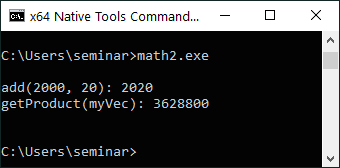
\includegraphics[width=0.8\textwidth]{content/5/chapter8/images/7.png}\\
在Windows上使用模块std.core
\end{center}

\subsubsubsection{8.1.3\hspace{0.2cm}执行器}

执行器在C++中的历史相当悠久,有关讨论早在2010年就开始了。关于细节,Detlef Vollmann在他的演讲\href{http://www.vollmann.ch/en/presentations/executors2018.pdf}{Finally Executors For C++}中给出了一个很好的概述。

我对执行器的介绍主要基于对执行器\href{http://www.open-std.org/jtc1/sc22/wg21/docs/papers/2018/p0761r2.pdf}{P0761}的设计建议,以及其正式描述\href{http://open-std.org/JTC1/SC22/WG21/docs/papers/2018/p0443r7.html}{P0443}。我还提到了相对较新的\href{http://open-std.org/JTC1/SC22/WG21/docs/papers/2018/p1055r0.pdf}{保守执行器提案 P1055}。

首先,啥是执行器?

执行器是C++中执行的基本构建块,并在执行中扮演类似的角色,例如C++中容器的分配器。许多关于执行器的建议已经发布,但还有很多设计决策仍然悬而未决。它们应该是C++23的一部分,但是可以更早地用于C++扩展标准。

执行器由关于在何处、何时,以及如何运行可调用对象的规则组成。

\begin{itemize}
\item 
Where: 可调用对象可以在内部或外部处理器上运行,结果可以从内部或外部处理器读取。

\item 
When: 可调用对象可以立即运行,也可以只是调度。

\item 
How: 可调用对象可以在CPU或GPU上运行,甚至可以以向量化的方式执行。
\end{itemize}

C++的并发性和并行性特性,很大程度依赖于执行器的构建块。这种依赖关系适用于现有的并发特性,例如\href{https://www.modernescpp.com/index.php/parallel-algorithm-of-the-standard-template-library}{并行算法的标准模板库},但也适用于新的并发特性,例如\href{https://www.modernescpp.com/index.php/std-future-extensions}{门闩和栅栏,协程,网络库,扩展的future},\href{https://www.modernescpp.com/index.php/transactional-memory}{事务性内存}或\href{https://www.modernescpp.com/index.php/task-blocks}{任务块}。

\hspace*{\fill} \\ %插入空行
\noindent
\textbf{8.1.3.1\hspace{0.2cm}一个例子}

下面的代码应该会给展示一个关于执行器的使用。

\hspace*{\fill} \\ %插入空行
\noindent
\textbf{8.1.3.1.1\hspace{0.2cm}使用执行器}

\begin{itemize}
\item 
使用std::async

\hspace*{\fill} \\ %插入空行
\noindent
\textbf{std::async中使用执行器}
\begin{lstlisting}[style=styleCXX]
// get an executor through some means
my_executor_type my_executor = ...

// launch an async using my executor
auto future = std::async(my_executor, [] {
	std::cout << "Hello world, from a new execution agent!" < '\n';
});
\end{lstlisting}

\item 
STL算法std::for\_each

\hspace*{\fill} \\ %插入空行
\noindent
\textbf{std::for\_each使用执行器}
\begin{lstlisting}[style=styleCXX]
// get an executor through some means
my_executor_type my_executor = ...

// execute a parallel for_each "on" my executor
std::for_each(std::execution::par.on(my_executor),
			  data.begin(), data.end(), func);
\end{lstlisting}
\end{itemize}

\hspace*{\fill} \\ %插入空行
\noindent
\textbf{8.1.3.1.2\hspace{0.2cm}获取执行器}

有多种可获取执行器。

\begin{itemize}
\item 
从static\_thread\_pool的执行上下文中获取

\begin{lstlisting}[style=styleCXX]
// create a thread pool with 4 threads
static_thread_pool pool(4);

// get an executor from the thread pool
auto exec = pool.executor();

// use the executor on some long-running task
auto task1 = long_running_task(exec);
\end{lstlisting}

\item 
从系统执行器中获取
\end{itemize}

若没有指定,系统执行器是默认执行器。

\begin{itemize}
\item 
从一个执行器适配器中获取

\begin{lstlisting}[style=styleCXX]
// get an executor from a thread pool
auto exec = pool.executor();

// wrap the thread pool's executor in a logging_executor
logging_executor<decltype(exec)> logging_exec(exec);

// use the logging executor in a parallel sort
std::sort(std::execution::par.on(logging_exec), my_data.begin(), my_data.end());
\end{lstlisting}

logging\_executor是池执行器的包装器。
\end{itemize}

\hspace*{\fill} \\ %插入空行
\noindent
\textbf{8.1.3.2\hspace{0.2cm}执行器的目的}

根据提案\href{http://open-std.org/JTC1/SC22/WG21/docs/papers/2018/p1055r0.pdf}{P1055},执行器的目标是什么呢?

\begin{itemize}
\item 
可批处理的:控制可调用对象转换的成本与其体积之间的权衡。

\item 
异构:允许可调用对象在异构上下文中运行并返回结果。

\item 
有序:指定调用可调用对象的顺序。目标包括顺序保证,如后进先出、FIFO先入先出执行、优先级或时间限制,甚至是顺序执行。

\item 
可控:可调用对象必须是针对特定计算资源的,可以延迟,甚至取消。

\item 
可持续:对于非阻塞提交的工作单元,需要来自工作单元的信号。这些信号必须指示结果是否可用、是否发生错误、可调用对象何时完成,或被调用者是否想要取消可调用对象。也应该可以显式地启动可调用对象或停止启动。

\item 
可分层:层次结构允许在不增加简单用例复杂性的情况下添加新功能。

\item 
可用:实现人员和用户的易用性应该是主要目标。
 
\item 
可组合:允许用户为不属于标准的特性扩展执行器。

\item 
最小化:执行器概念上不应该存在任何需要添加到其概念之上的东西。
\end{itemize}

\hspace*{\fill} \\ %插入空行
\noindent
\textbf{8.1.3.3\hspace{0.2cm}执行函数}

执行器提供一个或多个执行函数,用于从可调用对象创建执行代理。执行程序必须至少支持以下六个函数中的一个。

\begin{center}
执行器的函数
\end{center}

\begin{table}[H]
\centering
\begin{tabular}{lll}
\textbf{成员函数} & \textbf{基数} & \textbf{方向} \\ \hline
execute                  & 单个               & oneway             \\
twoway\_execute          & 单个               & twoway             \\
then\_execute            & 单个               & then               \\
bulk\_execute            & 批量                 & oneway             \\
bulk\_twoway\_execute    & 批量                 & twoway             \\
bulk\_then\_execute      & 批量                 & then              
\end{tabular}
\end{table}

每个执行函数都有两个属性:基数和方向。

\begin{itemize}
\item 
基数:
\begin{itemize}
\item 
单个: 创建一个执行代理

\item 
批量: 创建一组执行代理
\end{itemize}

\item 
方向:
\begin{itemize}
\item 
oneway: 创建执行代理,但不返回结果

\item
twoway: 创建执行代理并返回可用于等待执行完成的future

\item
then: 创建执行代理并返回可用于等待执行完成的future,执行代理在给定的future准备就绪后开始执行。
\end{itemize}
\end{itemize}

下面几行对执行函数进行了更正式的解释。

首先,引用单基数的情况:

\begin{itemize}
\item 
oneway执行函数是即发即忘的任务,非常类似于“即发即弃”,但它不会自动阻塞\href{https://www.modernescpp.com/index.php/the-special-futures}{future}的析构函数。

\item
twoway执行函数返回一个future,可以用它来获取结果。其行为类似于\href{https://www.modernescpp.com/index.php/promise-and-future}{std::promise},将返回相关std::future的句柄。

\item
then执行函数是一个延续,返回一个future,但是只有在提供的future准备就绪时,执行代理才会运行。
\end{itemize}

其次,批量基数的情况更复杂。这些函数创建一组执行代理,每个执行代理调用给定的可调用对象。它们返回工厂的结果,而不是执行代理调用的单个可调用f的结果。用户负责通过该工厂,消除正确结果的歧义。

\hspace*{\fill} \\ %插入空行
\noindent
\textbf{8.1.3.3.1\hspace{0.2cm}execution::require}

如何确保执行程序支持特定的执行函数?

特殊情况下,就会知道:

\hspace*{\fill} \\ %插入空行
\noindent
\textbf{使用执行函数execute的执行器}
\begin{lstlisting}[style=styleCXX]
void concrete_context(const my_oneway_single_executor& ex)
{
	auto task = ...;
	ex.execute(task);
}
\end{lstlisting}

一般情况下,可以使用函数execute::require来请求。

\hspace*{\fill} \\ %插入空行
\noindent
\textbf{需要单一和twoway执行函数的执行器}
\begin{lstlisting}[style=styleCXX]
template <typename Executor>
void generic_context(const Executor& ex)
{
	auto task = ...;
	
	// ensure .twoway_execute() is available with execution::require()
	execution::require(ex, execution::single, execution::twoway).twoway_execute(task\
	);
}
\end{lstlisting}

在这种情况下,执行器ex必须支持单基数和twoway执行。

\subsubsubsection{8.1.4\hspace{0.2cm}网络库}

C++23中的网络库基于Christopher M. Kohlhoff的\href{https://www.boost.org/doc/libs/1_75_0/doc/html/boost_asio.html}{boost::asio}库。该库的目标是网络和底层I/O编程。

下面的组件是网络库的一部分

\begin{itemize}
\item 
TCP, UDP和多路广播

\item 
客户机/服务器应用

\item 
更多并发连接的可扩展性

\item 
IPv4和IPv6

\item 
域名解析(DNS)

\item 
时钟
\end{itemize}

但是,以下组件不是网络库的一部分:

\begin{itemize}
\item 
网络协议的实现,如HTTP、SMTP或FTP

\item 
加密(SSL或TLS)

\item 
操作特定的多路复用接口,如select或轮询

\item 
支持实时

\item 
TCP/IP协议,如ICMP
\end{itemize}

由于支持了网络库,就可以直接实现一个回显服务器。

\hspace*{\fill} \\ %插入空行
\noindent
\textbf{一个简单的回显服务器}
\begin{lstlisting}[style=styleCXX]
template <typename Iterator>
void uppercase(Iterator begin, Iterator end) {
	std::locale loc("");
	for (Iterator iter = begin; iter != end; ++iter)
	*iter = std::toupper(*iter, loc);
}

void sync_connection(tcp::socket& socket) {
	try {
		std::vector<char> buffer_space(1024);
		while (true) {
			std::size_t length = socket.read_some(buffer(buffer_space));
			uppercase(buffer_space.begin(), buffer_space.begin() + length);
			write(socket, buffer(buffer_space, length));
		}
	}
	catch (std::system_error& e) {
		// ...
	}
}
\end{lstlisting}

服务器获取客户端套接字(第8行),读取文本(第12行),将文本转换为大写字母(第13行),并将文本发送回客户端(第14行)。

boost库有更多聊天或HTTP服务器的示例。此外,服务器可以同步运行(如程序中所示),也可以异步运行。






















